\documentclass[highlight, final]{jobim2017}
% Available options are:
% - showframe 
% - draft
% - final [default]

\usepackage[utf8]{inputenc}

% WARNING: already loaded packages:
% - hyperref
% - times
% - color
% - xspace
% - graphicx
% - fancyhdr
% - fancybox
% - indentfirst
% - geometry
% - babel (options english,francais) :
%   choose the language with \selectlanguage{<language>}


\pagestyle{empty}
\addtolength{\parskip}{0.4\baselineskip}

%% Title of the paper (required)
\title{Template for \jobim2017 Highlight [Titre/Title]}

%% List of authors (separated by the macro \and).
%% Authors can be followed by \inst{<n>} macro.
%% The <n> parameter of the \inst macro should correspond to the <n>th institution
%% (see macro \institute below).
\author{FirstName \textsc{LastName1}\inst{1} \and FirstName \textsc{LastName2}\inst{2} \and FirstName \textsc{LastName3}\inst{2}}

%% List of institutions (separated by the macro \and).
\institute{
 Laboratory, Address, zip code, Town, Country
 \and
 Laboratory, Address, zip code, Town, Country 
}

% email of the corresponding author
\corresponding{firstname.lastname1@email.fr}

% Enter the reference of your paper
\papername{Meert \textit{et al.} (2016) Unknown species discovered by metagenomics
  of frikandels. \textit{Annals of Improbable Research}. \url{http://dx.doi.org/11.0110/0111/111-1110-0001}}

%% Abstract of the paper (required).
\abstract{%
 The abstract of the paper (optional for short contributions) must be typeset
 in italic, with \emph{Times New Roman} 11-point font. The left and right margins
 must be set to 3cm. \textcolor{red}{350 words maximum.}
}

%% List of keywords of the paper (required).
\keywords{Some keywords, important, relevant. Five relevant keywords maximum. The keywords must be typeset in regular, 
with \emph{Times New Roman} 11-point font. The left and right margins must be set to 3cm.}

\begin{document}

 % Si vous écrivez en français, commentez la ligne suivante
\selectlanguage{english}
 % Si vous écrivez en francais, décommentez la ligne suivante...
 % \selectlanguage{francais}

   \maketitle

 \section{Introduction (\emph{Times New Roman} 12-point type, bold)}
 \label{sec:introduction}

This is the {\LaTeX} template for \jobim2017 proceedings.

The \textbf{Title:} \emph{Times New Roman} bold 14-point font, center

The \textbf{Authors names:} \emph{Times New Roman} 11-point font. Center as
well. Please typeset the last name(s) of author(s) in small caps, starting
with an uppercase first letter

The \textbf{Addresses:} Monospace 9-point font

The \textbf{Email:} Monospace 9-point font. Just give the email address of the corresponding author.

The \textbf{Paper reference:} \emph{Times New Roman} 10-point font, bold. First author, year, title, Journal, \textcolor{blue}{DOI link in blue}

\section{Document Structure (\emph{Times New Roman} 12-point type, bold)}
\label{sec:doc-struct}

The horizontal margins must be set to 2cm each, with no binding offset. The
vertical margins must be set to 2.5cm each. You can provide the
\verb+showframe+ option of the \LaTeXe\space class to see the page layout.

The \textbf{Text:} use \emph{Times New Roman} 11-point font and 6-point spacing between paragraphs.
Italics may be used to emphasize words in running text. Bold type and underlining should be avoided.
With these sizes, the interline distance should be set so that around 50 lines occur on a full-text
page.


\subsection{Page Numbering (\emph{Times New Roman} 11-point type, bold)}
\label{sec:page-numbering}

Pages must \textcolor{red}{NOT} be numbered. Final pagination will be set by
the editors of the proceedings.

\subsection{Figures and Photographs (\emph{Times New Roman} 11-point type, bold)}
\label{sec:figures-photographs}

Please produce your figures such that they display well in black \& white
mode, and integrate them into your text file. Please note that no figure will
be taken into account if not integrated in your text file.

Figures should be numbered and should have a
caption which should always be positioned under the figures. The final
sentence of a caption should end with a period. Please center the captions
between the margins and set them in
\emph{Times New Roman} 10-point font for the text (\figurename~\ref{fig:puzzle} shows an
example).

 \begin{figure}
   \begin{center}
     \setlength{\unitlength}{5mm}
     % if you have pdflatex installed, you can use pdf files as graphics
     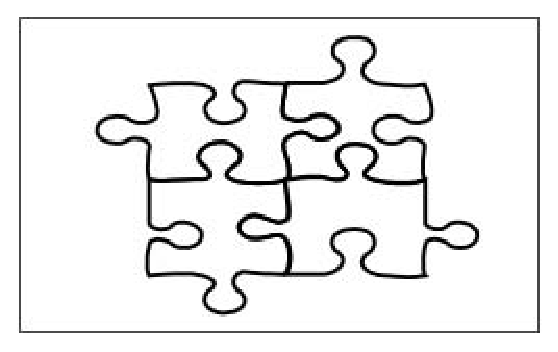
\includegraphics[height=4cm,width=6cm]{figs/fig1}
     % On the other hand, you must use eps files
     % 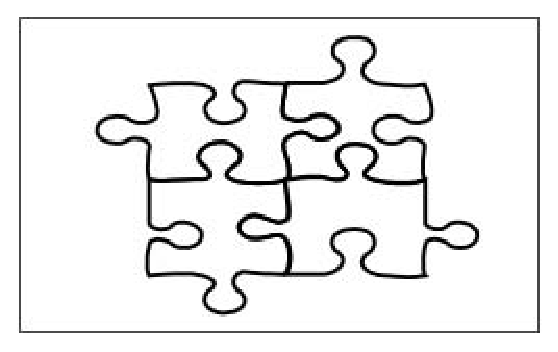
\includegraphics[height=4cm,width=6cm]{figs/fig1.eps}
   \end{center}
   \caption{Old \jobim puzzle (end of the 20th century).}
   \label{fig:puzzle}
 \end{figure}

\subsection{Tables (\emph{Times New Roman} 11-point type, bold)}
\label{sec:tables}

Table content should be in \emph{Times New Roman} 10-point font as well as their
captions. The rules used for the figures are also applied for the tables
(see \tablename~\ref{tab:exple} for example). Please note that no table will be
taken into account if not integrated in your text file.

\begin{table}[ht]
  \begin{center}
    \begin{tabular}{|l|c|c|c|c|c|c|}
      \hline
              & Col.1 & Col.2 & Col.3 & Col.4 & Col.5 & Col.6 \\
       \hline
       Row 1 &        &       &       &       &       &      \\
       \hline
       Row 2 &        &       &       &       &       &      \\
       \hline
       Row 3 &        &       &       &       &       &      \\
       \hline
       Row 4 &        &       &       &       &       &      \\
       \hline
    \end{tabular}
  \end{center}
  \caption{Example of a plain, dull, ordinary table for \jobim.}
  \label{tab:exple}
\end{table}

\section{Citations}
\label{sec:citations}

The list of references is headed
\emph{\refname}, it should be placed at the end of your
contribution. It should be in \emph{Times New Roman} 10-point font. Please do not
insert a page break before the list of references. For citations in the text,
please use square brackets \cite{Sokal1996} and consecutive ordered numbers
\cite{GastelDay2016,Cormode2012} in list of references.
Please find below examples on how to format references corresponding to
articles \cite{Sokal1996}, books \cite{GastelDay2016}, book chapters and proceedings
\cite{Cormode2012}.

\section{Warning} 
Note that the maximum length of \emph{Highlight} submission must not exceed \textcolor{red}{\emph{\JobimHighlightMaxPages{} pages}. A paper disregarding the
format described in this document will be rejected (even if it was previously accepted 
by the program committee).}

\begin{acknowledgements}
  \label{sec:acknowledgements}
  
 This work was supported by \jobim2017.
\end{acknowledgements}


 \bibliography{jobim_highlight}
 
\end{document}

